\chapter{مفاهیم پایه}

\section{مقدمه}

راه اندازی و استقرار سرویس در صنعت مخابرات به طور سنتی بر این اساس است که اپراتورهای شبکه سخت افزارهای اختصاصی فیزیکی و تجهیزات لازم برای هر کارکرد در سرویس را در زیرساخت خود مستقر کنند.
فراهم کردن نیازمندی هایی مانند پایداری و کیفیت بالا منجر به اتکای فراهم کنندگان سرویس بر سخت افزارهای اختصاصی می شود. 
این درحالی است که نیازمندی کاربران به سرویس های متنوع و عموما با عمرکوتاه و نرخ بالای ترافیک افزایش یافته است.
بنابراین فراهم کنندگان سرویس های باید مرتبا و به صورت پیوسته تجهیزات فیزیکی جدید را خریده، انبارداری کرده و مستقر کنند.
تمام این عملیات باعث افزایش هزینه های فراهم کنندگان سرویس می شود.
با افزایش تجهیزات، پیدا کردن فضای فیزیکی برای استقرار تجهیزات جدید به مرور دشوارتر می شود.
علاوه بر این باید افزایش هزینه و تاخیر ناشی از آموزش کارکنان برای کار با تجهیزات جدید را نیز در نظر گرفت.
بدتر این ‍که هر چه نوآوری سرویس‍ها و فناوری شتاب بیشتری می‍گیرد، چرخه عمر سخت‍افزارها کوتاه‍تر می‍شود که مانع از ایجاد نوآوری در سرویس های شبکه می شود.

در روش سنتی استقرار سرویس شبکه، ترافیک کاربر باید از تعدادی کارکرد شبکه به ترتیب معینی عبور کند تا یک مسیر پردازش ترافیک ایجاد شود.
در حال حاضر این کارکردها به صورت سخت افزاری به یکدیگر متصل هستند و ترافیک با استفاده از جداول مسیریابی به سمت آن ها هدایت می شود.
چالش اصلی این روش در این است که استقرار و تغییر ترتیب کارکردها دشوار است.
به عنوان مثال، به مرور زمان با تغییر شرایط شبکه نیازمند تغییر همبندی و یا مکان کارکردها برای سرویس دهی بهتر به کاربران هستیم که نیاز به جا به جایی کارکردها و تغییر جداول مسیریابی دارد.
در روش سنتی این کار سخت و هزینه بر است که ممکن است خطاهای بسیاری در آن رخ دهد.
از جنبه دیگر، تغییر سریع سرویس های مورد نظر کاربران نیازمند تغییر سریع در ترتیب کارکردها است که در روش فعلی این تغییرات به سختی صورت گیرد.
بنابراین اپراتورهای شبکه نیاز به شبکه های قابل برنامه ریزی و ایجاد زنجیره سرویس کارکردها به صورت پویا پیدا کرده اند.

دو فناوری برای پاسخگویی به این چالش‌ها مطحر شد:
مجازی‌سازی کارکرد شبکه یا \lr{NFV}
زنجیره‌سازی کارکردهای سرویس یا \lr{SFC}
هدف از
\lr{NFV}
این است که کاکردها بتوانند روی سخت‌افزارهای استاندارد اجرا شوند
تا نیاز به سخت‌افزارهای خاص منظوره کاهش یابد.
از طرف دیگر
\lr{SFC}
امکان تعریف زنجیره‌ی کارکردها به صورت پویا و در هر زمان را ارائه می‌کند که تغییر در زیرساخت فیزیکی را کاهش می‌دهد.

از آنجایی که از مفاهیم این فناوری ها برای طراحی و تعریف مساله در این رساله استفاده شده است، نیازمند آشنایی با مفاهیم ابتدایی و اصول اولیه آن ها خواهیم بود.

بنابراین در این فصل به صورت خلاصه اجزای این فناوری ها را مرور خواهیم کرد و کاربردها، چالش ها و مسائل تحقیقاتی که در هر یک از این معماری ها وجود دارد را مورد بررسی قرار خواهیم داد.

\section{مجازی‌سازی کارکرد شبکه}

مجازی‌‍سازی کارکرد شبکه اصل جداسازی کارکرد شبکه به وسیله انتزاع سخت افزاری مجازی از سخت افزاری است که بر روی آن اجرا می شود.
هدف مجازی سازی کارکرد شبکه تغییر روش اپراتورهای شبکه در طراحی شبکه با تکامل مجازی سازی استاندارد فناوری اطلاعات به منظور تجمیع تجهیزات شبکه در سرورهای استاندارد، سوییچ ها و ذخیره سازها با توان بالا است.
یک سرور استاندارد با توان بالا سروری است که توسط اجزای استاندارد شده \lr{IT}، مانند معماری \lr{x86}، ساخته شده و در تعداد بالایی، مانند میلیون، فروخته می شود.
ویژگی اصلی این سرورها این است که اجزای آن ها به راحتی از فروشندگان مختلف قابل خریداری و تعویض است.
این تجهیزات می توانند در مراکز داده، گره های شبکه، یا مکان کاربران انتهایی قرار بگیرند.

مزایا و اهداف اساسی که \lr{NFV} برای تحقق و دست‍یابی به آن‍ها شکل گرفته است عبارتند از:

\begin{itemize}
    \item
    کاهش هزینه‌های تجهیزات و مصرف انرژی از طریق تجمیع کارکردها بر روی سرورها و در نتیجه کاهش تعداد تجهیزات
    \item
    کاهش نیاز به آموزش کارکنان، افزایش دسترسی پذیری به سخت افزار و کاهش زمان بازیابی از خرابی سخت افزار به علت استفاده از سخت افزارهای استاندارد و عمومی
    \item
    افزایش سرعت عرضه محصول به بازار با کوتاه‍کردن چرخه نوآوری و تولید. در واقع \lr{NFV} به اپراتورهای شبکه کمک می‍کند تا چرخه بلوغ محصول را به اندازه قابل توجهی کاهش دهند.
    \item
    امکان‍پذیر بودن تعریف سرویس مورد نظر بر اساس نوع مشتری یا محل جغرافیایی. مقیاس سرویس‍ها می‍تواند به سرعت، بر اساس نیاز، گسترش یا کاهش یابد.
    \item
    تشویق به ایجاد نوآوری‍ و ارائه سرویس‍های جدید و دریافت جریان‍های درآمدی تازه با سرعت بالا و ریسک پایین.
    \item
    افزایش توانایی  مقابله با خرابی کارکردها، قابلیت به اشتراک گذری منابع بین کارکرد ها و پشتیابی از چند مشتری
\end{itemize}

سازمان‍های استانداردگذاری متعددی در استانداردسازی فناوری \lr{NFV} دخیل هستند که شاخص‍ترین آن‌ها موسسه استانداردهای مخابراتي اروپا (\lr{ETSI}) است.
در اواخر سال ۲۰۱۲،
\lr{ETSI NFV ISG}
توسط هفت اپراتور جهانی شبکه به منظور ارتقا ایده مجازی‌سازی کارکرد شبکه تأسیس شد.
\lr{NFV ISG}
تبدیل به یک بستر صنعتی اصلی برای توسعه چارچوب معماری \lr{NFV} و نیازمندی‍های آن شده است و اکنون بیش از ۲۵۰ سازمان با آن همکاری میکنند.
اسناد معماری \lr{NFV} به صورت عمومی و رایگان توسط \lr{ETSI NFV ISG} منتشر می شود.
ما در این رساله برای توصیف معماری \lr{NFV} از اسناد ارائه شده این سازمان استفاده می کنیم.

\section{معماری \lr{NFV}}

در این بخش مؤلفه‌های تشکیل‌دهنده معماری \lr{NFV} شرح داده می‍شوند.
هر یک از اجزای معماری می‍توانند توسط تولیدکنندگان متفاوتی تأمین شوند و به وسیله واسط هایی که توسط معماری \lr{NFV}
توصیف شده‌اند با یکدیگر در ارتباط باشند.

بنابراین معماری \lr{NFV} توصیف شده توسط \lr{ETSI} راه حلی با قابلیت مشارکت و هماهنگی چندین تولیدکننده مختلف را دارد.

با توجه به استاندارد \lr{ETSI} معماری \lr{NFV}
از سه عنصر کلیدی تشکیل شده است.
زیرساخت مجازی‌سازی کارکردهای شبکه،
کارکردهای مجازی شبکه‌ای و
\lr{NFV MANO}.
این اجزا در شکل \cref{fig.1} نمایش داده شده‌اند.

\begin{figure}[!h]
\center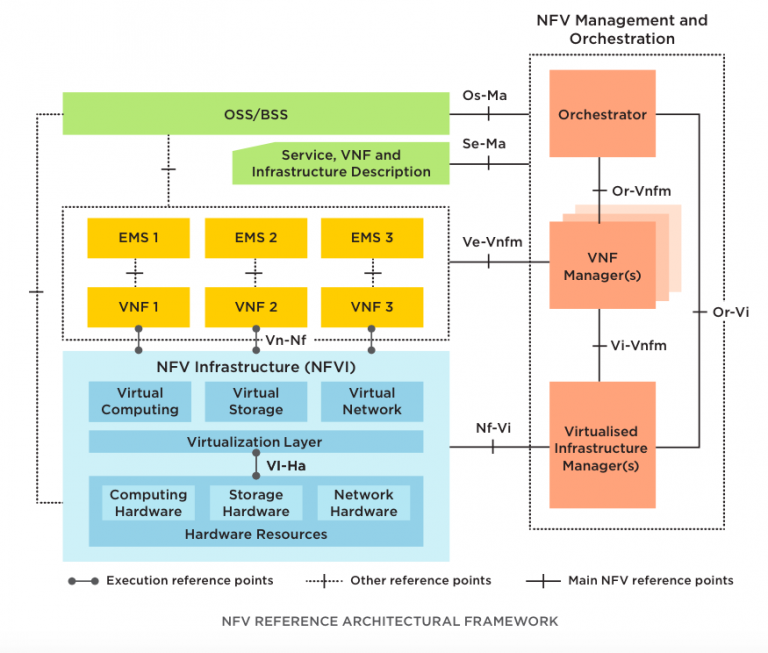
\includegraphics[scale=.5]{images/nfv-arch}
\caption{معماری مجازی‌سازی کارکردهای شبکه
}\label{fig.1}
\end{figure}

\begin{itemize}
    \item
    \lr{NFVI}: شامل منابع سخت افزاری و نرم افزاری لازم برای اجرای \lr{VNF} ها
    \item
    \lr{Service}: شامل \lr{VNF} ها که کارکردهای شبکه را پیاده سازی کرده اند، \lr{EMS} برای مدیریت \lr{VNF} ها و \lr{OSS/BSS} برای ارتباط با سیستم های مدیریت سنتی
    \item
    \lr{MANO}: که وظیفه مدیریت و هماهنگی سرویس ها و تخصیص منابع را برعهده دارد و از سه بخش \lr{NFVO}، \lr{VIM} و \lr{VNFM} تشکیل شده است.
\end{itemize}

\section{زیرساخت مجازی‌سازی کارکردهای شبکه}
زیرساخت مجازی‌سازی کارکردهای شبکه ترکیبی از منابع نرم‌افزاری و سخت‌افزاری است
که محیطی برای نصب
کارکردهای مجازی شبکه فراهم می‌آورد.
منابع سخت‌افزاری شامل منابع محاسباتی،
ذخیره‌سازها و شبکه
(شامل لینک‌ها و گره‌ها)
هستند
که پردازش، ذخیره‌سازی و ارتباط را
برای کارکردهای مجازی شبکه فراهم می‌آورند.
منابع مجازی انتزاعی از منابع شبکه‌ای، پردازشی و ذخیر‌ه‌سازی هستند.
به وسیله انتزاع از طریق لایه‌ی مجازی‌سازی (بر پایه‌ی \lr{hypervisor})
منابع سخت افزاری در اختیار کارکردهای مجازی
قرار می‌گیرند که این منابع شامل منابع محاسباتی، شبکه‌ای و ذخیره‌سازی می‌باشند.

در مراکز داده‌ای ممکن است منابع پردازشی و ذخیره‌سازی تحت عنوان یک یا چند
ماشین مجازی نمایش داده شوند در حالی که شبکه‌های مجازی از لینک‌ها و گره‌های مجازی تشکیل می‌شوند.
شبکه‌های مجازی پیش از بحث مجازی‌سازی کارکردهای شبکه مدنظر بوده‌اند و روی آن‌ها کار شده است.
در واقع از شبکه‌های مجازی در مراکز داده‌ای جهت فراهم آوردن شبکه‌های مختلف و مجزا که به کاربران مختلفی تعلق دارند
استفاده شده است. راه‌حل‌های مختلفی برای پیاده‌سازی این شبکه‌ها وجود دارد. در بحث مجازی‌سازی کارکردهای شبکه‌، زیرساخت ارتباطی
مورد نیاز 
برای کارکردهای مجازی از طریق همین شبکه‌های مجازی فراهم آورده می‌شود.
یعنی مسائلی که پیشتر در بحث جایگذاری شبکه‌های مجازی مطرح بود
امروز جزئی از مسائل جایگذاری زنجیره‌های کارکرد سرویس می‌باشند.

\section{کارکردهای مجازی شبکه}
یک کارکرد شبکه، یک بلوک عملیاتی در زیرساخت شبکه است که عملکرد رفتاری و رابط‌های ارتباط با خارج خوش تعریف دارد.
مثال‌هایی از کارکردهای شبکه می‌تواند شامل
\lr{DHCP}
یا
\lr{firewall}
و ... باشد.
با این توضیحات کارکرد مجازی شبکه، پیاده‌سازی یک کارکرد شبکه است
که می‌تواند روی منابع مجازی شده اجرا شود.
از هر کارکرد شبکه می‌توان نمونه‌سازی کرده و چند نمونه را در شبکه مستقر ساخت. 
این نمونه‌ها می‌توانند برای سرویس‌دهی به زنجیره‌های مختلف استفاده شوند. از آنجایی که 
هر نمونه توان پردازشی محدودی دارد با افزایش تعداد نمونه‌ها می‌توان توان پردازشی یک کارکرد را نیز افزایش داد.

\section{\lr{EM}}
این مولفه کارکردهای \lr{FCAPS} را برای \lr{VNF} ها انجام می دهد که شامل مدیریت خطا، پیکربندی، امنیت، حسابداری و کارایی برای کارکردی است که \lr{VNF} ارائه می دهد. این مولفه ممکن است آگاه از مجازی کارکرد باشد و با همکاری \lr{VNFM} عملکردهای خودش را انجام بدهد.

\section{\lr{OSS/BSS}}
این مولفه، ترکیبی از سایر بخش های عملکردهای اپراتور است که در چارچوب معماری \lr{NFV} ارائه شده از طرف \lr{ETSI} قرار نمیگیرند. به عنوان مثال می تواند شامل مدیریت سیستم های \lr{Legacy} باشد.

\section{\lr{NFV MANO}}
بر اساس چهارچوب پیشنهادی \lr{ETSI}
وظیفه‌ی \lr{NFV MANO} فراهم آوردن کارکردهای لازم
برای تدارک و فرآیند‌های مشابه مانند تنظیم کردن و ... کارکردهای مجازی شبکه است.
\lr{NFV MANO} شامل هماهنگ کننده و مدیریت کننده چرخه‌ی زندگی
منابع سخت‌افزاری و نرم‌افزاری که مجازی‌سازی زیرساخت را پشتیبانی می‌کنند، است.
هر زنجیره نیاز دارد که حداقل توسط یک \lr{VNFM} مدیریت شود
تا مثلا خطاهای آن را تحت نظر قرار دهد و در صورت نیاز در قسمت دیگری از شبکه استقرار یابد.
مساله‌ی جایگذاری زنجیره‌ها بسیار مورد مطالعه قرار گرفته است، اما در این بین توجه لازم به نیاز این زنجیره‌ها به یک
\lr{VNFM}
صورت نپذیرفته است.
